\subsection{Fixed-point theory} 
A fixed-point of a function is an element in the domain of that function such that the function maps to itself for that element. Fixed-point theory goes hand in hand with lattice theory which we introduce first.
\subsubsection{Lattices}
We introduce definitions for ordering and lattices taken from \cite{birkhoff1940lattice}.
\begin{definition}
	A partial order is a binary relation $x \leq y$ on set $S$ where for all $x,y,z \in S$ we have:
	\begin{itemize}
		\item $x \leq x$. (Reflexive)
		\item If $x \leq y$ and $y \leq x$, then $x=y$. (Antisymmetric)
		\item If $x \leq y$ and $y \leq z$, then $x \leq z$. (Transitive)
	\end{itemize}
\end{definition}

\begin{definition}
	A partially ordered set is a set $S$ and a partial order $\leq$ for that set, we denote a partially ordered set by $\langle S, \leq \rangle$.
\end{definition}

\begin{definition}
	Given partially ordered set $\langle P,\leq \rangle$ and subset $X \subseteq P$. An upper bound to $X$ is an element $a \in P$ such that $x \leq a$ for every $x\in X$. A least upper bound to $X$ is an upper bound $a \in P$ such every other upper bound is larger or equal to $a$.
	
	The term least upper bound is synonymous with the term supremum.
\end{definition}
\begin{definition}
	Given partially ordered set $\langle P,\leq \rangle$ and subset $X \subseteq P$. A lower bound to $X$ is an element $a \in P$ such that $a \leq x$ for every $x\in X$. A greatest lower bound to $X$ is a lower bound $a \in P$ such that every other lower bound is smaller or equal to $a$.
	
	The term greatest lower bound is synonymous with the term infimum.
\end{definition}

\begin{definition}
	A lattice is a partially ordered set where any two of its elements have a supremum and an infimum.
\end{definition}

\begin{definition}
	A complete lattice is a partially ordered set in which every subset has a supremum and an infimum.
\end{definition}

\begin{definition}
	A function $f : D \rightarrow D'$ is monotonic, also called order preserving, if for all $x \in D$ and $y \in D$ it holds that if $x \leq y$ then $f(x) \leq f(y)$.
\end{definition}
\subsubsection{Fixed-points}
Fixed-points are formally defined as follows:
\begin{definition}
	Given function $f : D \rightarrow D$ the value $x \in D$ is a fixed point for $f$ if and only if $f(x) = x$.
\end{definition}
\begin{definition}
	Given function $f : D \rightarrow D$ the value $x \in D$ is the least fixed point for $f$ if and only if $x$ is a fixed point for $f$ and every other fixed point for $f$ is greater or equal to $x$.
\end{definition}
\begin{definition}
	Given function $f : D \rightarrow D$ the value $x \in D$ is the greatest fixed point for $f$ if and only if $x$ is a fixed point for $f$ and every other fixed point for $f$ is less or equal to $x$.
\end{definition}
The Knaster-Tarski theorem states that least and greatest fixed points exist for some domain and function given that a few conditions hold.
The theorem, as written down by Tarski \cite{tarski1955}, states:
\begin{theorem}[Knaster-Tarski\cite{tarski1955}]
	\label{the_knaster_tarski}
	Let
	\begin{itemize}
		\item $\langle A, \leq \rangle$ be a complete lattice,
		\item $f$ be an increasing function on $A$ to $A$,
		\item $P$ be the set of all fixpoints of f.
	\end{itemize}
	Then the set $P$ is not empty and the system $\langle P, \leq \rangle$ is a complete lattice; in particular we have 
	\[ \sup P = \sup \{ x\ |\ f(x) \geq x \} \in P \]
	and
	\[ \inf P = \inf \{ x\ |\ f(x) \leq x \} \in P \]
\end{theorem}

\subsection{Model verification}
Behaviour of a software system can be modelled in a \textit{labelled transition system} (LTS). An LTS consists of states in which the system can find itself and transitions between states. An state in an LTS represents a state in the system and a transition represents the possible state change of a system. Transitions are labelled with actions that indicate what kind of change is happening. Formally we define an LTS as follows.
\begin{definition}[\cite{Groote}]
	\label{def_lts}
	A labelled transition system (LTS) is a tuple $M = (S, Act, trans, s_0)$, where:
	\begin{itemize}
		\item $S$ is a finite set of states,
		\item $Act$ a set finite of actions,
		\item $trans \subseteq S \times Act \times S$ is the transition relation with $(s,a,s') \in trans$ denoted by $s \xrightarrow a s'$,
		\item $s_0 \in S$ is the initial state.
	\end{itemize}
\end{definition}

An LTS is usually depicted as a graph where the vertices represent the states, the edges represent the transitions, the labels next to the edges represent the actions and an edge with no origin vertex indicates the initial state. Such a representation is depicted in the example below.
\begin{example}[\cite{FamBasedModelCheckingWithMCRL2}]
	We consider the behaviour of a coffee machine that accepts a coin after which it serves a standard coffee. This can be repeated infinitely often. 
	
	The behaviour can be modelled as an LTS that has two states: in the initial state it is ready to accept a coin and in the second state it is ready to serve a standard coffee. We introduce two actions: \textit{ins}, which represents a coin being inserted, and \textit{std}, which represents a standard coffee to be served. We get the following LTS which is also depicted in Figure \ref{fig:coffeemachinebasiceurolts}.
	\[ (\{s_1,s_2\},\{std,ins\},\{(s_1,ins,s_2),(s_2,std,s_1)\},s_1)\]
	\begin{figure}[h]
		\centering
		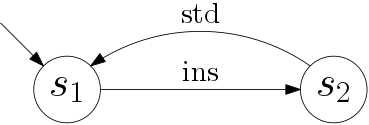
\includegraphics[scale=0.3]{Examples/CoffeeMachine/BasicEuroLTS}
		\caption[Coffee machine LTS]{Coffee machine LTS $C$}
		\label{fig:coffeemachinebasiceurolts}
	\end{figure}
\end{example}

LTSs might be non-deterministic meaning that if from a state there might be multiple transitions that can be taken, moreover multiple transitions with the same action can be taken. This is depicted in the example below.

\begin{example}
	We extend the coffee machine example where at some point the coffee machine can be empty and needs a fill before the system is ready to receive a coin again. This LTS is depicted in Figure \ref{fig:coffeemachineundeterministic}. When the \textit{std} transition is taken from state $s_2$ it is non-determined in which states the system ends.
	\begin{figure}[h]
		\centering
		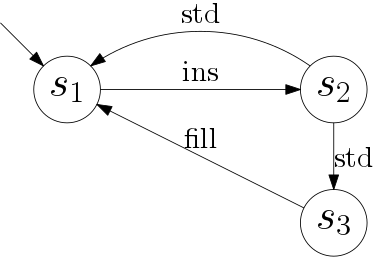
\includegraphics[scale=0.3]{Examples/CoffeeMachine/NonDeterministicEuroLTS}
		\caption[Coffee machine LTS]{Coffee machine with non-deterministic behaviour}
		\label{fig:coffeemachineundeterministic}
	\end{figure}
\end{example}


A system can be verified by checking if its behaviour adheres to certain requirements. The behaviour can be modelled in an LTS. Requirements can be expressed in a temporal logic, with a temporal logic we can express certain propositions with a time constraint such as \textit{always}, \textit{never} or \textit{eventually}. For example (relating to the coffee machine example) we can express the following constraint: "After a coin is inserted the machine always server a standard coffee immediately afterwards". The most expressive temporal logic is the modal $\mu$-calculus. A modal $\mu$-calculus formula is expressed over a set of actions and a set of variables.

We define the syntax of the modal $\mu$-calculus below. Note that we define the syntax in the positive form, ie. no negations.
\begin{definition}[\cite{Groote}]
	\label{def_mu_syntax}
	A modal $\mu$-calculus formula over the set of actions $Act$ and a set of variables $\mathcal{X}$ is defined by
	\[ \varphi = \top\ |\ \bot\ |\ X\ |\ \varphi \vee \varphi\ |\ \varphi \wedge \varphi\ |\ \langle a \rangle \varphi\ |\ [a]\varphi\ |\ \mu X.\varphi\ |\ \nu X.\varphi \]
	with $a \in Act$ and $X \in \mathcal{X}$. 
\end{definition}
The modal $\mu$-calculus contains boolean constants $\top$ and $\bot$, propositional operators $\vee$ and $\wedge$, modal operators $\langle \, \rangle$ and $[ \, ]$ and fixpoint operators $\mu$ and $\nu$. Variable $X \in \mathcal{X}$ \textit{occurs free} in formula $\phi$ if and only if $X$ is not a sub-formula of $\mu X.\phi'$ or of $\nu X.\phi'$ in $\phi$. A formula is \textit{closed} if and only if there are no free occurring variables.

A formula can be interpreted in the context of an LTS, such an interpretation results in a set of states in which the formula holds. Given formula $\varphi$ we define the interpretation of $\varphi$ as $\llbracket \varphi \rrbracket ^\eta  \subseteq S$ where $\eta : \mathcal{X}\rightarrow 2^S$ maps variables to a value. We can modify the a value of $\eta$ assign $S'$ to variable $X$, we write $\eta[X:=S'](X) = S'$.
\begin{definition}
	\label{def_mu_sem} For LTS $(S, Act, trans, s_0)$ we inductively define the interpretation of a modal $\mu$-calculus formula $\varphi$, notation
	$\llbracket \varphi \rrbracket^\eta$, where $\eta : \mathcal{X} \rightarrow \mathcal{P}(S)$ is a logical variable valuation, as a set of states
	where $\varphi$ is valid, by:
	\begin{align*}
	&\llbracket {\top} \rrbracket^\eta &&= S\\
	&\llbracket {\bot} \rrbracket^\eta &&= \emptyset\\
	&\llbracket \varphi_1 \wedge \varphi_2 \rrbracket^\eta &&= \llbracket \varphi_1 \rrbracket^\eta \cap \llbracket \varphi_2 \rrbracket^\eta \\
	&\llbracket \varphi_1 \vee \varphi_2 \rrbracket^\eta &&= \llbracket \varphi_1 \rrbracket^\eta \cup \llbracket \varphi_2 \rrbracket^\eta\\
	&\llbracket \langle a \rangle \varphi \rrbracket^\eta &&= \{s \in S|\exists_{s' \in S} s \xrightarrow {a} s' \wedge s' \in \llbracket \varphi \rrbracket^\eta\}\\
	&\llbracket [ a ] \varphi \rrbracket^\eta &&= \{s \in S|\forall_{s' \in S} s \xrightarrow {a} s' \implies s' \in \llbracket \varphi \rrbracket^\eta\}\\
	&\llbracket \mu X. \varphi \rrbracket^\eta &&= \bigcap\{f \subseteq S | f \supseteq \llbracket \varphi \rrbracket^{\eta[X:=f]}\}\\
	&\llbracket \nu X. \varphi \rrbracket^\eta &&= \bigcup\{f \subseteq S | f \subseteq \llbracket \varphi \rrbracket^{\eta[X:=f]}\}\\
	&\llbracket X \rrbracket^\eta &&= \eta(X)
	\end{align*}
\end{definition}
Since there are no negations in the syntax we find that every modal $\mu$-calculus formula is monotone, ie. if we have for $U \subseteq S$ and $U' \subseteq S$ that $U \subseteq U'$ then $\llbracket \varphi \rrbracket^{\eta[X:=U]} \subseteq \llbracket \varphi \rrbracket^{\eta[X:=U']}$ for any variable $X \in \mathcal{X}$. Using the Knaster-Tarski theorem (theorem \ref{the_knaster_tarski}) we find that the least and greatest fixed-points always exist.

Given closed formula $\varphi$, LTS $M = (S, Act, trans, s_0)$ and $s \in S$ we say that formula $\varphi$ holds for $M$ in state $s$ if and only if $s \in \llbracket \varphi \rrbracket^\eta$, we write $(M,s) \models \varphi$. If and only if formula $\varphi$ holds for $M$ in the initial state we say that formula $\varphi$ holds for $M$ and we write $M \models \varphi$. 

\begin{example}[\cite{FamBasedModelCheckingWithMCRL2}]
	Consider the coffee machine example we seen earlier in Figure \ref{fig:coffeemachinebasiceurolts} and formula $\varphi = \nu X. \mu Y([inst]Y \wedge [std]X)$ which states that action \textit{std} must occur infinitely often over all runs. Obviously this holds for the coffee machine, therefore we have $C \models \varphi$.
\end{example}

\subsection{Parity games}
Verifying LTSs against a modal $\mu$-calculus formula can be done by solving a \textit{parity game}. This is done by translating an LTS in combination with a formula to a parity game, the solution of the parity game provides the information needed to conclude if the model satisfies the formula. This relation is depicted in figure \ref{fig:ltsverificationusingpg}. This technique is well known and well studied, in this section we will first look at parity games, the translation from LTS and formula to a parity game and finally what we can do with this technique to verify FTS.
\begin{figure}[h]
	\centering
	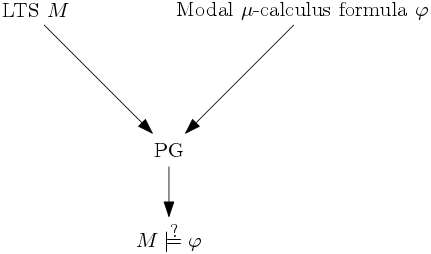
\includegraphics[scale=0.5]{Diagrams/LTSVerificationUsingPG}
	\caption[LTS verification using PG]{LTS verification using PG}
	\label{fig:ltsverificationusingpg}
\end{figure}

\begin{definition}
	\label{def_PG}\cite{Bradfield2018}
	A parity game (PG) is a tuple $(V, V_0, V_1, E, \Omega)$, where:
	\begin{itemize}
		\item $V = V_0 \cup V_1$ and $V_0 \cap V_1 = \emptyset$,
		\item $V_0$ is the set of vertices owned by player $0$,
		\item $V_1$ is the set of vertices owned by player $1$, 
		\item $E \subseteq V \times V$ is the edge relation,
		\item $\Omega :  V \rightarrow \mathbb{N}$ is a priority assignment.
	\end{itemize}
\end{definition}
A parity game is played by players 0 and 1. We write $\alpha \in \{0,1\}$ to denote an arbitrary player. We write $\overline{\alpha}$ to denote $\alpha$'s opponent, ie. $\overline{0} = 1$ and $\overline{1} = 0$.

A play starts with placing a token on vertex $v \in V$. Player $\alpha$ moves the token if the token is on a vertex owned by $\alpha$, ie. $v \in V_\alpha$. The token can be moved to $w \in V$, with $(v,w) \in E$. A series of moves results in a sequence of vertices, called a path. For path $\pi$ we write $\pi_i$ to denote the $i^{\text{th}}$ vertex in path $\pi$. A play ends when the token is on vertex $v \in V_\alpha$ and $\alpha$ can't move the token anywhere, in this case player $\overline{\alpha}$ wins the play. If the play results in an infinite path $\pi$ then we determine the highest priority that occurs infinitely often in this path, formally
\[ \max\{ p \ |\ \forall_j \exists_i j < i \wedge p = \Omega(\pi_i) \}\] 
If the highest priority is odd then player $1$ wins, if it is even player $0$ wins.
\begin{figure}[h]
	\centering
	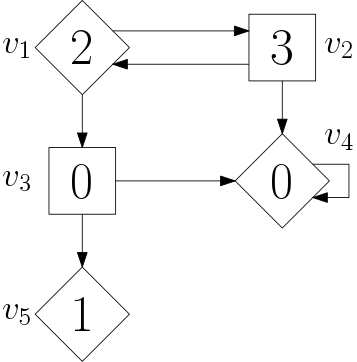
\includegraphics[scale=0.3]{Examples/SimplePG/PG}
	\caption[Parity game example]{Parity game example}
	\label{fig:simplepgpg}
\end{figure}

Figure \ref{fig:simplepgpg} shows an example of a parity game. We usually depict the vertices owned by player $0$ by diamonds and vertices owned by player $1$ by boxes, the priority is depicted inside the vertices. If the game starts by placing a token on $v_1$ we can consider the following exemplary paths:
\begin{itemize}
	\item $\pi = v_1v_3v_5$ is won by player $1$ since player $0$ can't move at $v_5$.
	\item $\pi = (v_1v_2)^\omega$ is won by player $1$ since the highest priority occurring infinitely often is 3.
	\item $\pi = v_1v_3(v_4)^\omega$ is won by player $0$ since the highest priority occurring infinitely often is $0$.
\end{itemize}


A strategy for player $\alpha$ is a function $\sigma : V^*V_\alpha \rightarrow V$ that maps a path ending in a vertex owned by player $\alpha$ to the next vertex. Parity games are positionally determined \cite{Bradfield2018}, therefore a strategy $\sigma: V_\alpha \rightarrow V$ that maps the current vertex to the next vertex is sufficient. 

A strategy $\sigma$ for player $\alpha$ is winning from vertex $v$ iff any play that results from following $\sigma$ results in a win for player $\alpha$. The graph can be divided in two partitions $W_0 \subseteq V$ and $W_1 \subseteq V$, called winning sets. Iff $v \in W_\alpha$ then player $\alpha$ has a winnings strategy from $v$. Every vertex in the graph is either in $W_0$ or $W_1$ \cite{Bradfield2018}. Furthermore finite parity games are decidable \cite{Bradfield2018}.

\subsubsection{Verifying LTSs using parity games}
A parity game can be created from a combination of an LTS and a modal $\mu$-calculus formula. To do this we introduce some auxiliary definitions regarding the modal $\mu$-calculus.

First we introduce the notion of unfolding, a fixpoint formula $\mu X . \varphi$ can be unfolded resulting in formula $\varphi$ where every occurrence of $X$ is replaced by $\mu X . \varphi$, denoted by $\varphi [ X:= \mu X . \varphi]$. A fixpoint formula is equivalent to its unfolding \cite{Bradfield2018}, ie. for some LTS $[\![\mu X . \varphi]\!]^\eta = [\![\varphi[X:=\mu X . \varphi]]\!]^\eta$. The same holds for the fixpoint operator $\nu$.

Next we define the Fischer-Ladner closure for a closed $\mu$-calculus formula 
\cite{STREETT1989249,FISCHER1979194}. The Fischer-Ladner closure of $\varphi$ is the set $\textit{FL}(\varphi)$ of closed formula's containing at least $\varphi$. Furthermore for every formula $\psi$ in $\textit{FL}(\varphi)$ it holds that for every direct subformula $\psi'$ of $\psi$ there is a formula in $\textit{FL}(\varphi)$ that is equivalent to $\psi'$.
\begin{definition}
	\label{def_FLClosure}
	The Fischer-Ladner closure of closed $\mu$-calculus formula $\varphi$ is the smallest set $\textit{FL}(\varphi)$ satisfying the following constraints:
	\begin{itemize}
		\item $\varphi \in \textit{FL}(\varphi)$,
		\item if $\varphi_1 \vee \varphi_2 \in \textit{FL}(\varphi)$ then $\varphi_1 ,\varphi_2 \in \textit{FL}(\varphi)$,
		\item if $\varphi_1 \wedge \varphi_2 \in \textit{FL}(\varphi)$ then $\varphi_1 ,\varphi_2 \in \textit{FL}(\varphi)$,
		\item if $\langle a \rangle \varphi' \in \textit{FL}(\varphi)$ then $\varphi' \in \textit{FL}(\varphi)$,
		\item if $[ a ] \varphi' \in \textit{FL}(\varphi)$ then $\varphi' \in \textit{FL}(\varphi)$,
		\item if $\mu X . \varphi' \in \textit{FL}(\varphi)$ then $\varphi'[X:= \mu X . \varphi'] \in \textit{FL}(\varphi)$ and
		\item if $\nu X . \varphi' \in \textit{FL}(\varphi)$ then $\varphi'[X:= \nu X . \varphi'] \in \textit{FL}(\varphi)$.
		
	\end{itemize}
\end{definition}

Finally we define alternating depth.
\begin{definition}\cite{Bradfield2018}
	The dependency order on bound variables of $\varphi$	is the smallest partial order such that $X \leq_\varphi Y$ if $X$ occurs free in $\sigma Y. \psi$ . The alternation depth of a $\mu$-variable X in formula $\varphi $ is the maximal length of a chain $X_1 \leq_\varphi  \dots \leq_\varphi X_n$ where $X = X_1$, variables $X_1, X_3, \dots$ are $\mu$-variables and variables $X_2, X_4, \dots$ are $\nu$-variables. The alternation depth of a $\nu$-variable is defined similarly. The alternation depth of formula $\varphi$, denoted $adepth(\varphi)$, is the maximum of the alternation depths of the variables bound in $\varphi$, or zero if there are no fixpoints.
\end{definition}
Consider the example formula $\varphi = \nu X. \mu Y. ([ins]Y \wedge [std] X)$ which states that for an LTS with $Act = \{ ins, std\}$ the action \textit{std} must occur infinitely often over all runs. Since $X$ occurs free in $\mu Y. ([ins] Y \wedge [std]X)$ we have $adepth(Y) = 1$ and $adepth(X) = 2$. As shown in \cite{Bradfield2018} it holds that formula $\mu X. \psi$ has the same alternation depth as its unfolding $\psi[X:=\mu X. \psi]$. Similarly for the greatest fixpoint.



We can now define the transformation from an LTS and a formula to a parity game.
\begin{definition}
	\label{def_LTS2PG}\cite{Bradfield2018}
	LTS2PG($M, \varphi$) converts LTS $M = (S, Act, trans, s_0)$ and closed formula $\varphi$ to a PG $(V, V_0, V_1, E, \Omega)$.
	
	A vertex in the parity game is represented by a pair $(s, \psi)$ where $s \in S$ and $\psi$ is a modal $\mu$-calculus formula. We will create a vertex for every state with every formula in the Fischer-Ladner closure of $\varphi$. We define the set of vertices:
	\[ V = S \times \textit{FL}(\varphi) \]
	
	We create the parity game with the smallest set $E$ such that:
	\begin{itemize}
		\item $V = V_0 \cup V_1$,
		\item $V_0 \cap V_1 = \emptyset$ and
		\item for every $v = (s, \psi) \in V$ we have:
		\begin{itemize}
			\item If $\psi = \top$ then $v \in V_1$.
			\item If $\psi = \bot$ then $v \in V_0$.
			\item If $\psi = \psi_1 \vee \psi_2$ then:
			\subitem $v \in V_0$,
			\subitem $(v, (s,\psi_1)) \in E$ and
			\subitem $(v, (s,\psi_2)) \in E$.
			\item If $\psi = \psi_1 \wedge \psi_2$ then:
			\subitem $v \in V_1$,
			\subitem $(v, (s,\psi_1)) \in E$ and
			\subitem $(v, (s,\psi_2)) \in E$.
			\item If $\psi = \langle a \rangle \psi'$ then $v \in V_0$ and for every $s \xrightarrow{ a} s'$ we have $(v, (s', \psi')) \in E$.
			\item If $\psi = [ a ] \psi'$ then $v \in V_1$ and for every $s \xrightarrow{ a} s'$ we have  $(v, (s', \psi')) \in E$.
			\item If $\psi = \mu X. \psi'$ then $(v, (s, \psi'[X:=\mu X. \psi'])) \in E$.
			\item If $\psi = \nu X. \psi'$ then $(v, (s, \psi'[X:=\nu X. \psi'])) \in E$.
		\end{itemize}
	\end{itemize}
	Since the Fischer-Ladner formula's are closed we never get the case $\psi = X$.
	
	Finally we have $\Omega(s, \psi) = \begin{cases}
	2 \lfloor adepth(X) / 2 \rfloor & \text{if } \psi = \nu X. \psi'\\
	2 \lfloor adepth(X) / 2 \rfloor + 1 & \text{if } \psi = \mu X. \psi'\\
	0 & \text{otherwise}
	\end{cases}$
\end{definition}
\begin{figure}[h]
	\centering
	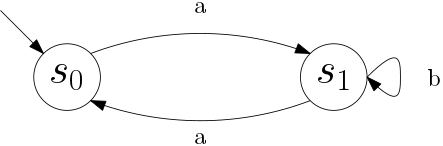
\includegraphics[scale=0.3]{Examples/ExamleVerification/LTSprojempty}
	\caption[LTS $M$]{LTS $M$}
	\label{fig:exverltsprojempty}
\end{figure}\begin{figure}[h]
	\centering
	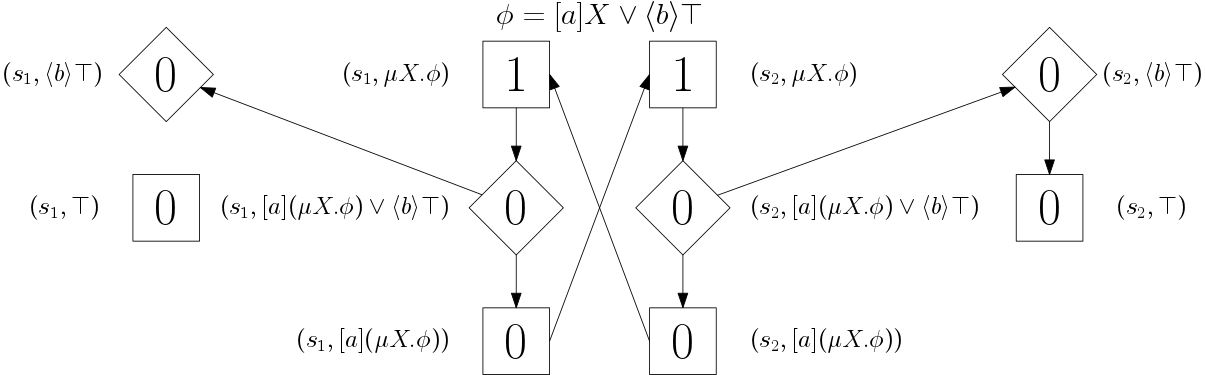
\includegraphics[scale=0.3]{Examples/ExamleVerification/PG}
	\caption[Parity game $LTS2PG(M, \varphi)$]{Parity game $LTS2PG(M, \varphi)$}
	\label{fig:exverpg}
\end{figure}
Consider LTS $M$ in figure \ref{fig:exverltsprojempty} and formula $\varphi = \mu X.([a]X \vee \langle b \rangle \top)$ expressing that on any path reached by $a$'s we can eventually do a $b$ action. We will use this as a working example in the next few sections. The resulting parity game is depicted in figure \ref{fig:exverpg}. Solving this parity game results in the following winning sets:%
\begin{align*}
W_0 = \{& (s_1, \mu X.\phi),\\
& (s_1, [a](\mu X. \phi) \vee \langle b \rangle \top),\\
& (s_1, [a](\mu X. \phi)),\\
& (s_1, \top),\\
& (s_2, \mu X.\phi),\\
& (s_2, [a](\mu X. \phi) \vee \langle b \rangle \top),\\
& (s_2, [a](\mu X. \phi)),\\
& (s_2, \langle b \rangle \top),\\
& (s_2, \top)
\}\\
W_1 = \{& (s_1, \langle b \rangle \top )\}
\end{align*}
With the strategies $\sigma_0$ for player $0$ and $\sigma_1$ for player $1$ being (vertices with one outgoing edge are omitted):
\begin{align*}
\sigma_0 = \{
&(s_1, [a](\mu X. \phi) \vee \langle b \rangle \top) \mapsto (s_1, [a] (\mu X. \phi)), \\
&(s_2, [a](\mu X. \phi) \vee \langle b \rangle \top) \mapsto (s_2, \langle b \rangle \top) \} \\
\sigma_1 = \{&\} \\
\end{align*}

State $s$ in LTS $M$ only satisfies $\varphi$ iff player $0$ has a winning strategy from vertex $(s, \varphi)$. This is formally stated in the following theorem which is proven in \cite{Bradfield2018}.
\begin{theorem}
	\label{the_LTS_PG_REL}Given LTS $M = (S, Act, trans, s_0)$, modal $\mu$-calculus formula $\varphi$ and state $s \in S$ it holds that $(M, s) \models \varphi$ iff $s \in W_0$ for the game $LTS2PG(M, \varphi)$.
\end{theorem}

\subsubsection{Parity game algorithms}
We inspect two existing parity game algorithms which are used in the collective VPG algorithms. First Zielonka's recursive algorithm which is well studied and generally considered to be one of the best performing parity game algorithm \cite{Oink,SolvingPGInPractice}. We also inspect the fixed-point iteration algorithm which tends to perform well for model-checking problems with a low number of distinct priorities \cite{BDDSolvingPG}.

\paragraph{Zielonka's recursive algorithm}
First we consider Zielonka's recursive algorithm, created from the constructive proof given in \cite{ZIELONKA1998135}, which solves total PGs. Pseudo code is presented in algorithm \ref{alg_zlnk_org}. Zielonka's recursive algorithm has a worst-case time complexity of $O(e*n^d)$.
\begin{algorithm}
	\caption{$\textsc{RecursivePG}(\textit{PG } G = (V,V_0,V_1, E, \Omega))$}
	\label{alg_zlnk_org}
	\begin{algorithmic}[1]
		\State $m \gets \min\{ \Omega(v)\ |\ v \in V\}$
		\State $h \gets\max\{ \Omega(v)\ |\ v \in V\}$
		\If{$h = m$ or $V = \emptyset$}
		\If{$h$ is even or $V = \emptyset$}
		\State \Return $(V,\emptyset)$
		\Else
		\State \Return $(\emptyset, V)$
		\EndIf
		\EndIf
		\State $\alpha \gets 0$ if $h$ is even and $1$ otherwise
		\State $U \gets \{v \in V\ |\ \Omega(v) = h\}$
		\State $A \gets \alpha\textit{-Attr}(G, U)$
		\State $(W_0', W_1') \gets \textsc{RecursivePG}(G \backslash A)$
		\If{$W_{\overline{\alpha}}' =\emptyset$}
		\State $W_\alpha \gets A \cup W_\alpha'$
		\State $W_{\overline{\alpha}} \gets \emptyset$
		\Else
		\State $B \gets \overline{\alpha}\textit{-Attr}(G,W_{\overline{\alpha}}')$
		\State $(W_0'', W_1'') \gets \textsc{RecursivePG}(G \backslash B)$
		\State $W_\alpha \gets W_\alpha''$
		\State $W_{\overline{\alpha}} \gets W_{\overline{\alpha}}'' \cup B$
		\EndIf
		\State \Return $(W_0, W_1)$
	\end{algorithmic}
\end{algorithm}

The algorithm works for solving $G$ by taking the set of vertices with the highest priority and choosing player $\alpha$ such that $\alpha$ has the same parity as the highest priority. Next the algorithm finds all the vertices such that player $\alpha$ can force the play to one of these high priority vertices. Next this set of vertices is removed from the game and the resulting subgame is solved recursively. This subgame returns winning sets $W'_0$ and $W'_1$. Vertices in set $W'_{\overline{\alpha}}$ are won by player $\overline{\alpha}$ in the subgame but are also won by player $\overline{\alpha}$ in $G$. The algorithm tries to find all the vertices in $G$ such that player $\overline{\alpha}$ can force the play to a vertex in $W'_{\overline{\alpha}}$ and therefore winning the game. We now have a set of vertices that are definitely won by player $\overline{\alpha}$ in game $G$. In the rest of the game player $\alpha$ can keep the play from $W'_{\overline{\alpha}}$ so the algorithm solves the rest of the game recursively to find the complete winning sets for game $G$.

A complete explanation of the algorithm can be found in \cite{ZIELONKA1998135}, we do introduce definitions for the attractor set and for subgames. 

An attractor set is a set of vertices $A \subseteq V$ calculated for player $\alpha$ given set $U \subseteq V$ where player $\alpha$ has a strategy to force the play starting in any vertex in $A \backslash U$ to a vertex in $U$.

\begin{definition}\cite{ZIELONKA1998135}
	\label{def_attr}Given parity game $G = (V,V_0,V_1,E,\Omega)$ and a non-empty set $U \subseteq V$ we define $\alpha\textit{-Attr}(G,U)$ such that
	\[U_0 = U \]
	For $i \geq 0$:
	\begin{align*}
	U_{i+1} = U_i\cup
	&\{v \in V_\alpha\ |\ \exists v' \in V : v' \in U_i \wedge (v,v') \in E \}\\
	\cup &\{v \in V_{\overline{\alpha}}\ |\ \forall v' \in V :(v,v') \in E \implies v' \in U_i \}
	\end{align*}
	Finally:
	\[\alpha\textit{-Attr}(G,U) = \bigcup_{i \geq 0} U_i \]
\end{definition}

\begin{figure}
	\centering
	\begin{subfigure}{1\textwidth}
		\centering
		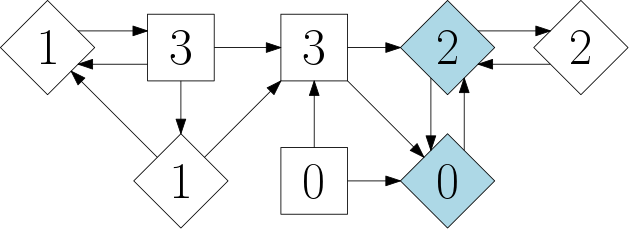
\includegraphics[scale=0.4]{Examples/Attr/Attr0}
		\caption{Set $U = U_0$}
	\end{subfigure}\\
	\begin{subfigure}{1\textwidth}
		\centering
		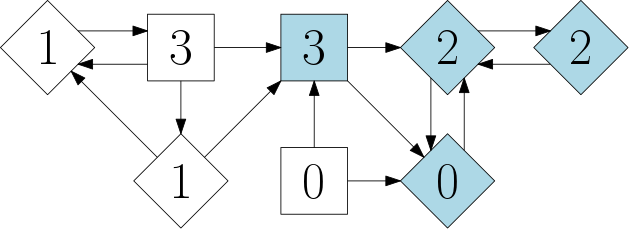
\includegraphics[scale=0.4]{Examples/Attr/Attr1}
		\caption{Set $U_1$}
	\end{subfigure}\\
	\begin{subfigure}{1\textwidth}
		\centering
		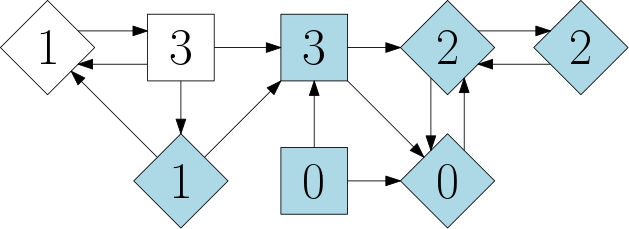
\includegraphics[scale=0.4]{Examples/Attr/Attr2}
		\caption{Set $U_2 = 0\textit{-Attr}(G,U)$}
	\end{subfigure}
	\caption{Game $G$ showing the attractor calculation for $0\textit{-Attr}(G,U)$}
	\label{fig:AttrCalcExample}
\end{figure}
Figure \ref{fig:AttrCalcExample} shows an example parity game in which an attractor set is calculated for player $0$. For set $U_2$ no more vertices can be attracted so we found the complete attractor set.

The algorithm also creates subgames, where a set of vertices is removed from a parity game to create a new parity game.

\begin{definition}\cite{ZIELONKA1998135}
	\label{def_org_subgame}
	Given a parity game $G = (V,V_0,V_1, E,\Omega)$ and $U \subseteq V$ we define the subgame $G \backslash U$ to be the game $(V', V_0', V_1', E', \Omega)$ with:
	\begin{itemize}
		\item $V' = V \backslash U$,
		\item $V_0' = V_0 \cap V'$,
		\item $V_1' = V_1 \cap V'$ and
		\item $E' = E \cap (V' \times V')$.
	\end{itemize}
\end{definition}

Note that a subgame is not necessarily total, however the recursive algorithm always creates subgames that are total (shown in \cite{ZIELONKA1998135}).

\paragraph{Fixed-point iteration algorithm}
Parity games can be solved by solving an alternating fixed-point formula, as shown in \cite{WALUKIEWICZ2002311}. We will consider PG $G = (V,V_0,V_1, E, \Omega)$ with $d$ distinct priorities. We can apply \textit{priority compression} to make sure every priority in $G$ maps to a value in $\{0,\dots,d-1\}$ or $\{1, \dots, d\}$ \cite{SolvingInPractice,FPITE}. We assume without loss of generality that the priorities map to $\{0,\dots,d-1\}$ and that $d-1$ is even. 

Consider the following formula
\[ S(G = (V,V_0,V_1,E,\Omega)) = \nu Z_{d-1}. \mu Z_{d-2}. \dots . \nu Z_0. F_0(Z_{d-1},\dots,Z_0) \]
with
\[ F_0(Z_{d-1},\dots,Z_0) = \{ v \in V_0\ |\ \exists_{w\in V} (v,w) \in E \wedge Z_{\Omega(w)} \} \cup \{ v \in V_1\ |\ \forall_{w\in V} (v,w) \in E \implies Z_{\Omega(w)} \} \]
where $Z_i \subseteq V$. The formula $\nu X. f(X)$ solves the greatest fixed-point of $X$ in $f$, similarly $\mu X.f(X)$ solves the least fixed-point of $X$ in $f$.

To understand the formula we consider sub-formula $\nu Z_0. F_0(Z_{d-1},\dots,Z_0)$. This formula holds for vertices from which player $0$ can either force the play into a node with priority $i > 0$ for which $Z_i$ holds or the player can stay in vertices with priority $0$ indefinitely. The formula $\mu Z_0. F_0(Z_{d-1},\dots,Z_0)$ holds for vertices from which player $0$ can force the play into a node with priority $i > 0$, for which $Z_i$ holds in finitely many steps. By alternating fixed-points the formula allows infinitely many stays in even vertices and finitely many stays in odd vertices. For an extensive treatment we refer to \cite{WALUKIEWICZ2002311}.

We further inspect formula $S$. Given game $G$, consider the following subformula's:
\[ S^{d-1}(Z_{d-1}) = \mu Z_{d-2}.S^{d-2}(Z_{d-2})\]
\[ S^{d-2}(Z_{d-2}) = \nu Z_{d-3}.S^{d-3}(Z_{d-3})\]
\begin{center}
	\dots
\end{center}
\[ S^{0}(Z_0) = F_0(Z_{d-1},\dots,Z_0)\]
The fixed-point variables are all elements of $2^V$, therefore we have for every subformula the following type:
\[ S^i(Z_i) : 2^V \rightarrow 2^V \]
Furthermore, since $V$ is finite, the partially ordered set $\langle 2^V, \subseteq \rangle$ is a complete lattice.

Finally every subformula is $S^i(Z_i)$ is monotonic, ie. if $S^i(Z_i) \geq S^i(Z_i')$ then $Z_i \geq Z_i'$.

Fixed-point formula's can be solved by fixed-point iteration. As shown in \cite{Emerson:1986:MCP:900378} we can calculate $\mu X.f(X)$, where $f$ is monotonic in $X$ and $X \in 2^V$, by iterating $X$:
\[ \mu X.f(X) = \bigcup_{i \geq 0} X^i \]
where $X^i = f(X^{i-1})$ for $i > 0$ and $X^0 \subseteq \mu X.f(X)$. So picking the smallest value possible for $X_0$ will always correctly calculate $\mu X. f(X)$.

Similarly we can calculate fixed-point $\nu X.f(X)$ when $f$ is monotonic in $X$ by iterating $X$.
\[ \nu X.f(X) = \bigcap_{i \geq 0} X^i \]
where $X^i = f(X^{i-1})$ for $i > 0$ and $X^0 \supseteq \nu X.f(X)$. So picking the largest value possible for $X_0$ will always correctly calculate $\nu X. f(X)$.

Since every subformula is monotonic and maps from a value in $2^V$ to another value in $2^V$ we can apply fixed-point iteration to solve the subformula's, we choose initial values $\emptyset$ for least fixed-point variables and $V$ for greatest fixed-point variables.

An algorithm to perform the iteration is presented in \cite{FPITE} and shown in algorithm \ref{alg_FPITEorg}. This algorithm has a worst-case time complexity of $O(e * n ^d)$.
\begin{algorithm}
	\caption{Fixed-point iteration}
	\label{alg_FPITEorg}
	\begin{multicols}{2}
		\begin{algorithmic}[1]
			\Function{FPIter}{$G = (V, V_0, V_1, E, \Omega)$}
			\For{$i \gets d-1,\dots,0$}
			\State $\textsc{Init}(i)$
			\EndFor
			\Repeat
			\State $Z_0'\gets Z_0$
			\State $Z_0 \gets \textsc{Diamond}() \cup \textsc{Box}()$
			\State $i \gets 0$
			\While{$Z_i=Z_i' \wedge i < d-1$}
			\State $i \gets i+1$
			\State $Z_i' \gets Z_i$
			\State $Z_i \gets Z_{i-1}$
			\State $\textsc{Init}(i-1)$
			\EndWhile
			\Until{$i = d-1 \wedge Z_{d-1} = Z_{d-1}'$}
			\State \Return $(Z_{d-1},V\backslash Z_{d-1})$
			\EndFunction
		\end{algorithmic}\bigskip\bigskip
		\begin{algorithmic}[1]
			\Function{Init}{$i$}
			\State $Z_i \gets \emptyset$ if $i$ is odd, $V$ otherwise
			\EndFunction
		\end{algorithmic}\bigskip
		\begin{algorithmic}[1]
			\Function{Diamond}{}
			\State \Return $\{ v \in V_0\ |\ \exists_{w\in V} (v,w) \in E \wedge w \in Z_{\Omega(w)}\}$
			\EndFunction
		\end{algorithmic}\bigskip
		\begin{algorithmic}[1]
			\Function{Box}{}
			\State \Return $\{ v \in V_1\ |\ \forall_{w\in V} (v,w) \in E \implies w \in Z_{\Omega(w)}\}$
			\EndFunction
		\end{algorithmic}
	\end{multicols}
\end{algorithm}

\subsubsection{Locally solving parity games}
Parity games can be solved \textit{globally} or \textit{locally}; globally solving a parity game means that for every vertex in the game it is determined who the winner is. Locally solving a parity game means that for a specific vertex in the game it is determined who the winner is. For some applications of parity games, including model checking, there is a specific vertex that needs to be solved to solve the model checking problem so locally solving the parity game is sufficient for solving the original problem.

Most parity game algorithms are concerned with global solving, when talking about solving a PG we talk about globally solving it unless stated otherwise. 

\subsection{Symbolically representing sets}
A set can straightforwardly be represented by a collection containing all the elements that are in the set. We call this an \textit{explicit} representation of a set. We can also represent sets \textit{symbolically} in which case the set of elements is represented by some sort of formula. A typical way to represent a set symbolically is through a boolean formula encoded in a \textit{binary decision diagram} \cite{BDD_book,Handbook_BDD_Chapter}. For example the set $S = \{0,1,2,4,5,7 \}$ can be expressed by boolean formula:
\[ F(x_2,x_1,x_0) = (x_2 \vee \neg x_1 \vee \neg x_0) \wedge (\neg x_2 \vee \neg x_1 \vee x_0) \]
where $x_0,x_1$ and $x_2$ are boolean variables. The formula gives the following truth table:\\
\begin{center}
	\begin{tabular}{|c|c|}
		\hline 
		$\mathbf{x_2x_1x_0}$ & $\mathbf{F(x_2,x_1,x_0)}$ \\ 
		\hline 
		000 & 1 \\ 
		\hline 
		001 & 1 \\ 
		\hline 
		010 & 1 \\ 
		\hline 
		011 & 0 \\ 
		\hline 
		100 & 1 \\ 
		\hline 
		101 & 1 \\ 
		\hline 
		110 & 0 \\ 
		\hline 
		111 & 1 \\ 
		\hline 
	\end{tabular} 
\end{center}
The function $F$ defines set $S'$ in the following way: $S' = \{x_2x_1x_0\ |\ F(x_2,x_1,x_0) = 1 \}$. As we can see set $S'$ and $S$ represent the same numbers. We can perform set operations on sets represented as boolean functions by performing logical operations on the functions. For example, given boolean formula's $f$ and $g$ representing sets $V$ and $W$ the formula $f \wedge g$ represents set $V \cap W$.

Boolean functions can efficiently be represented in BDDs, for a comprehensive treatment of BDDs we refer to \cite{BDD_book,Handbook_BDD_Chapter}. We will note here that given $x$ boolean variables and two boolean functions encoded as BDDs we can perform binary operations $\vee,\wedge$ on them in $O(2^{2x})=O(m^2)$ where $m = 2^x$ is the maximum set size that can be represented by $x$ variables \cite{BDD_running_time,Handbook_BDD_Chapter}. The running time specifically depends on the size of the decision diagrams, in general if the boolean functions are simple then the size of the decision diagram is also small and operations can be performed quickly.